O Filtro de Kalman (KF) é uma técnica de estimação ótima para sistemas lineares com ruídos gaussianos. Nele, a função densidade de probabilidade do estado estimado é representada por uma gaussiana, 
Equação \ref{eq:moments-gaussian-probabilistic-distribution}, parametrizada pelos momentos centrais média e covariância. O KF foi desenvolvido simultaneamente em 1958 por Peter Swerling e em 1960 por Rudolf Kalman \cite[p.~40]{thrun2005probabilistic}. Apesar de sua otimalidade ser garantida apenas para sistemas lineares, ele é aplicado em sistemas não lineares também. Para isso, é feita uma aproximação linear em torno da estimativa do estado atual do sistema, utilizando-se expansão por série de Taylor, e a premissa de que os termos de ordem maior ou igual a dois são desprezíveis.

\begin{equation}
  \pr{\bvec{x}} = \eta \exp\parentheses{-\frac{1}{2} 
  \parentheses{\bvec{x} - \mean{}}^T \cov{}^{-1}\parentheses{\bvec{x} - \mean{}}}
  \label{eq:moments-gaussian-probabilistic-distribution}
\end{equation}

Essa técnica derivada do KF para sistemas não lineares é conhecida como Filtro de Kalman Estendido (EKF). O EKF é muito utilizado em aplicações reais, pois a grande maioria dos sistemas reais são não lineares, como o movimento de um robô diferencial, por exemplo. Além disso, o modelo de medida do sensor é, muitas vezes, uma função não linear do estado do sistema.

Neste capítulo, serão descritas as alterações necessárias no EKF clássico para que ele possa ser aplicado na resolução do problema SLAM, estimando a pose do robô e a posição das \textit{landmarks}, o que é conhecido como EKF-SLAM. Além disso, também serão abordadas técnicas decorrentes do EKF-SLAM, como EIF-SLAM (Filtro de Informação Estendido) e SEIF-SLAM (Filtro de Informação Estendido Esparso), sendo esta última a técnica de estimação utilizada neste trabalho.

\section{Filtro de Kalman Estendido}
\label{sec:ekf}
Para que seja possível estimar o estado de um sistema utilizando-se KF, é 
necessário conhecer duas equações: a primeira, denominada modelo do sistema, 
modela a transição de estado do sistema a partir do estado anterior e da entrada aplicada, Equação \ref{eq:system-model}; a segunda, chamada de modelo de medida, relaciona o estado do sistema com a medida, gerada pelo sensor, Equação \ref{eq:measurement-model}. 
\begin{align}
  \bsubvec{x}{t} &= \mb{g}(\bsubvec{x}{t-1}, \bsubvec{u}{t}) + \mb{\epsilon}_t
  \label{eq:system-model}\\
  \bsubvec{y}{t} &= \mb{h}(\bsubvec{x}{t}) + \mb{\delta}_t
  \label{eq:measurement-model}
\end{align}
\newcommand{\EKFSystemModel}{$\mb{g}(\cdot, \cdot)$}
Como o modelo do sistema \EKFSystemModel{}, e o modelo de medida \measurementModel{} não são exatos, suas incertezas e erros de modelagem são aproximados por ruídos gaussianos $\mb{\epsilon}_t \sim \normal{\bvec{0}}{\bsubvec{R}{t}}$ e $\mb{\delta}_t \sim \normal{\bvec{0}}{\bsubvec{Q}{t}}$. Quando \EKFSystemModel{} e/ou \measurementModel{} não são lineares, o EKF pode ser utilizado para estimar o estado 
do sistema. 

As Equações de \ref{eq:ekf-prediction} até \ref{eq:ekf-estimate-error-covariance} definem o EKF \footnote{O leitor pode estanhar a Equação \ref{eq:ekf-estimate-error-covariance} do erro da estimativa. Normalmente ela é escrita na forma $\cov{t} = (\bvec{I} - \bsubvec{K}{t} \bsubvec{H}{t}) \predcov{t}$, porém de acordo com \citeonline[p.~ 73]{lewis2017optimal}, a forma em \ref{eq:ekf-estimate-error-covariance} é uma alternativa melhor na presença de erros de arredondamento, e é frequentemente utilizada em implementações de software.} para o sistema não linear acima. Sendo $\bsubvec{G}{t}$ o jacobiano do modelo do sistema no estado estimado atualizado prévio $\mean{t-1}$ e $\bsubvec{H}{t}$ é o jacobiano do modelo de medida no estado estimado predito $\predmean{t}$.
\begin{align}
  \predmean{t} &= \mb{g}(\mean{t-1}, \bsubvec{u}{t})
  \label{eq:ekf-prediction}\\
  \predcov{t} &= \bsubvec{G}{t}\cov{t-1}\bsubvecT{G}{t} + \bsubvec{R}{t}
  \label{eq:ekf-prediction-error-covariance}\\
  \bsubvec{z}{t} &= \bsubvec{y}{t} - \mb{h}(\predmean{t})
  \label{eq:ekf-inovation} \\
  \bsubvec{Z}{t} &= \bsubvec{H}{t}\predcov{t}\bsubvecT{H}{t} + \bsubvec{Q}{t}
  \label{eq:ekf-inovation-covariance} \\
  \bsubvec{K}{t} &=   \predcov{t}\bsubvecT{H}{t} \bsubvec{Z}{t}^{-1}
  \label{eq:ekf-gain}\\
  \mean{t} &= \predmean{t} + \bsubvec{K}{t} \bsubvec{z}{t}
  \label{eq:ekf-update}\\
  \cov{t} &= \predcov{t} - \bsubvec{K}{t}\bsubvec{Z}{t}\bsubvecT{K}{t}
  \label{eq:ekf-estimate-error-covariance}
\end{align}
Em que: 
\begin{itemize}
  \item $\predcov{t}$ é a matriz de covariância do estado predito
  \item $\bsubvec{z}{t}$ é o vetor de inovação
  \item $\bsubvec{Z}{t}$ é a matriz de covariância da inovação, também conhecido por matriz de inovação
  \item $\bsubvec{K}{t}$ é o Ganho de Kalman
  \item $\cov{t}$ é a matriz de covariância do estado atualizado
\end{itemize}
Porém, a resolução do problema SLAM utilizando o EKF, não é uma aplicação 
direta das Equações acima. São necessárias algumas alterações, pois em SLAM o vetor de medidas tem tamanho variável. Esses detalhes e outras particularidades da aplicação do EKF em SLAM serão tratados na próxima Seção.

\section{EKF-SLAM}
Para aplicar o EKF na solução de SLAM, é necessário entender 
como o vetor de estados $\bvec{x}$ é composto (aqui o subíndice $t$ é omitido, pois não é importante para esta discussão). Como tanto a pose do 
robô, quanto o mapa são estimados, o vetor de estados é composto por ambos como apresentado na Equação \ref{eq:slam-state-vector}, abaixo.
\begin{equation}
  \bvec{x} = \begin{bmatrix}
    \bsubvec{x}{\mathrm{r}} \\
    \bsubvec{x}{\mathrm{m}}
  \end{bmatrix}
  \label{eq:slam-state-vector}
\end{equation}
O vetor $\bsubvec{x}{\mathrm{m}}$, que representa o mapa, é composto pela posição $(x, y)$ das \textit{landmarks} identificadas. 
Seu tamanho é variável e cresce à medida que o robô navega pelo ambiente e 
mede novas \textit{landmarks}.
\begin{equation}
  \bsubvec{x}{\mathrm{m}} = \begin{bmatrix}
    m_x^1\\
    m_y^1\\
    \vdots\\
    m_x^n\\
    m_y^n
  \end{bmatrix}
  \label{eq:feature-map}
\end{equation}

Utilizando a definição do vetor de estados do EKF-SLAM acima (Equação \ref{eq:slam-state-vector}), as próximas três Seções (\ref{sec:ekf-slam-prediction}, \ref{sec:ekf-slam-update} e \ref{sec:ekf-slam-landmark-insertion}) descrevem as alterações necessários e/ou desejáveis no EKF para sua aplicação em SLAM. O algoritmo completo pode ser encontrado no Apêndice \ref{app:alg-ekf-slam}.

\subsection{EKF-SLAM: Predição (Movimento do robô)}
\label{sec:ekf-slam-prediction}
Em SLAM apenas uma parte do vetor de estados é variante no tempo, a pose do 
robô. Isso significa que apenas a porção $\bsubvec{x}{\mathrm{r}}$ é alterada pela entrada $\bvec{u}$, logo o modelo do sistema consiste apenas no modelo de 
movimento do robô $\mb{g}_\mathrm{r}$ concatenado com as posições das \textit{landmarks}:
\begin{equation}
  \bsubvec{x}{t} = \begin{bmatrix}
    \mb{g}_\mathrm{r}(\bsubvec{x}{\mathrm{r}, \,t-1}, \bsubvec{u}{t}) \\
    \bsubvec{x}{\mathrm{m}}
  \end{bmatrix} + \begin{bmatrix} 
      \mb{\epsilon}_{\mathrm{r}, \,t} \\
      \bvec{0}
  \end{bmatrix}
  \label{eq:slam-prediction}
\end{equation}
Portanto, o passo de predição do vetor de média do estado do EKF-SLAM torna-se:
\begin{equation}
  \predmean{t} = \begin{bmatrix}
    \mb{g}_\mathrm{r}(\mean{\mathrm{r}, \,t-1}, \bsubvec{u}{t}) \\
      \mean{\mathrm{m}}
  \end{bmatrix}
\end{equation}
Em termos de implementação, isso significa que apenas as componentes e seus respectivos endereços na memória da 
pose são modificadas no vetor de estados. Dessa forma, o passo de predição do 
vetor de estados do EKF-SLAM 2D tem complexidade $\bigO{3}$ (constante), enquanto no EKF 
essa complexidade é $\bigO{n}$, onde $n$ é o tamanho do vetor de estados.

A matriz de covariância, $\cov{}$, também é parcialmente atualizada, pois o jacobiano do sistema na Equação \ref{eq:slam-prediction} possui forma esparsa:
\newcommand{\slamsystemjacobian}{
  \bsubvec{G}{t} = \begin{bmatrix}
    \bsubvec{G}{t}^{\mathrm{r}} & \bvec{0} \\
    \bvec{0} & \bvec{I}
  \end{bmatrix}
}
\begin{equation}
  \slamsystemjacobian
  \label{eq:slam-system-jacobian}
\end{equation}
Então, a equação do erro de predição do EKF, em \ref{eq:ekf-prediction-error-covariance}, torna-se:
\renewcommand{\arraystretch}{1.5}
\begin{equation}
\begin{aligned}
  \predcov{t} &= \begin{bmatrix}
    \bsubvec{G}{t}^\mathrm{r} & \bvec{0} \\
    \bvec{0} & \bvec{I}
  \end{bmatrix} \cov{t-1}  \begin{bmatrix}
    \bsubvec{G}{t}^\mathrm{r} & \bvec{0} \\
    \bvec{0} & \bvec{I}  
  \end{bmatrix}^T + \begin{bmatrix}
      \bsubvec{R}{t}^{\mathrm{r}}  & \bvec{0} \\ \bvec{0} & \bvec{0}
    \end{bmatrix} \\
  &= \begin{bmatrix}
    \bsubvec{G}{t}^\mathrm{r} & \bvec{0} \\
    \bvec{0} & \bvec{I}
  \end{bmatrix} 
  \begin{bmatrix}
    \cov{t-1}^{\mathrm{rr}} & \cov{t-1}^{\mathrm{rm}} \\
    \cov{t-1}^{\mathrm{mr}} & \cov{\mathrm{mm}}
  \end{bmatrix}  
  \begin{bmatrix}
    \bsubvec{G}{t}^\mathrm{r} & \bvec{0} \\
    \bvec{0} & \bvec{I}  
  \end{bmatrix}^T + \begin{bmatrix}
      \bsubvec{R}{t}^{\mathrm{r}} & \bvec{0} \\ \bvec{0} & \bvec{0}
    \end{bmatrix} \\
  &= \begin{bmatrix}
    \bsubvec{G}{t}^\mathrm{r} \cov{t-1}^\mathrm{rr} \brac{\bsubvec{G}{t}^\mathrm{r}}^T + \bsubvec{R}{t}^{\mathrm{r}}&  \bsubvec{G}{t}^\mathrm{r} \cov{t-1}^\mathrm{rm}\\
    \cov{t-1}^\mathrm{mr}\brac{\bsubvec{G}{t}^\mathrm{r}}^T & \cov{\mathrm{mm}} 
  \end{bmatrix} 
\end{aligned}
\label{eq:ekf-slam-prediction-error-covariance}
\end{equation}
\renewcommand{\arraystretch}{1.0}
A complexidade dessa operação é da ordem de $\bigO{n}$ por conta do termo $\bsubvec{G}{t}^\mathrm{r} \cov{t-1}^\mathrm{rm}$, enquanto no caso geral do EKF em que o jacobiano $\bsubvec{G}{t}$ é denso, essa complexidade é $\bigO{n^{2.376}}$, que é a complexidade da multiplicação de matrizes $n \times n$ \cite{coppersmith1987matrix}. A Figura 
\ref{fig:ekfslam-prediction} ilustra as porções do vetor de estados e da 
matriz de covariância modificadas no passo de predição do EKF-SLAM.

\begin{figure}[h]
  \centering
  \includestandalone[width=.45\textwidth]{figs/ekfslam-prediction}
  \caption[Elementos do vetor média e da matriz de covariância alterados no passo de predição do Filtro de Kalman Estendido de um sistema SLAM]{Partes modificadas do vetor de média do estado e da matriz de covariância durante o movimento do robô. O vetor de média do estado é representado pela barra na esquerda, e a matriz de covariância pelo quadrado na direita. As partes modificadas, em tons de cinza, correspondem ao estado do robô $\mean{\mathrm{r}}$  e sua autocovariância $\cov{\mathrm{rr}}$ (cinza escuro), e às covariâncias cruzadas, $\cov{\mathrm{rm}}$ e $\cov{\mathrm{mr}}$, entre o robô e o mapa (cinza claro). Note que as partes correspondentes ao mapa, $\mean{\mathrm{m}}$ e $\cov{\mathrm{mm}}$, 
  permanecem inalteradas (branco). Adaptado de \citeonline[p.~10]{jsola}.}
  \label{fig:ekfslam-prediction}
\end{figure}


\subsection{EKF-SLAM: Atualização}
\label{sec:ekf-slam-update}
Assim como na predição, no passo de atualização há algumas particularidades 
que devem ser levadas em conta no EKF-SLAM. Ao contrário de um sistema convencional, em SLAM o vetor de medidas é variável, seu tamanho depende da 
quantidade de \textit{landmarks} que vão sendo avistadas pelo robô enquanto 
ele navega pelo ambiente. Ou seja, no EKF-SLAM o vetor de medidas é sempre 
``incompleto''. Normalmente, a inovação $\bsubvec{z}{t}$ é computada para cada 
medida de maneira individual e é denotada por $\bsubvec{z}{t}^j$.
\begin{equation}
  \bsubvec{z}{t}^j = \bsubvec{y}{t}^j - \mb{h}^j(\predmean{t})
  \label{eq:ekf-slam-innovation}
\end{equation}
Além disso, como o jacobiano do modelo de medida na Equação \ref{eq:measurement-model-jacobian-full} é esparso, a covariância da inovação é computada por:
\renewcommand{\arraystretch}{1.5}
\begin{equation}
  \bsubvec{Z}{t}^j = \begin{bmatrix}
    \bsubvec{H}{\mathrm{r}}^j & \bsubvec{H}{\mathrm{m}}^j
  \end{bmatrix}
  \begin{bmatrix}
    \predcov{\mathrm{rr}} & \predcov{\mathrm{rm^j}} \\
    \predcov{\mathrm{rm^j}}^T & \predcov{\mathrm{m^j m^j}}
  \end{bmatrix}
  \begin{bmatrix}
    \bsubvec{H}{\mathrm{r}}^j \\ \bsubvec{H}{\mathrm{m}}^j
  \end{bmatrix} + \bsubvec{Q}{t}
  \label{eq:ekf-slam-innovation-covariance}
\end{equation}
\renewcommand{\arraystretch}{1.0}
As dimensões do vetor inovação e das matrizes na equação acima são constantes e dependem apenas da dimensão da pose do robô e da dimensão da medida. 
Portanto, aqui as complexidades ao se computar a inovação $\bsubvec{z}{t}^j$ e de sua covariância $\bsubvec{Z}{t}^j$ são constantes, enquanto no EKF essas complexidades são $\bigO{m}$ e $\bigO{nm^2}$, respectivamente, onde $m$ é o tamanho do vetor de medidas. Cabe enfatizar que, aqui, esse cálculo de complexidade constante deve ser repetido para cada observação presente no vetor de medidas, ou seja, no EKF-SLAM as computações da
inovação e sua covariância possuem complexidade linear na quantidade de medidas obtidas.

A computação do ganho do filtro Kalman $\bsubvec{K}{t}$ também é influenciado pelo 
tamanho constante da matriz de covariância da inovação ($2\times 2$, no caso deste trabalho), Equação \ref{eq:ekf-slam-innovation-covariance}, e pela esparsidade do jacobiano do modelo de medida, na Equação \ref{eq:measurement-model-jacobian-full}. Ademais, se todos os cálculos triviais de multiplicação por zero não forem feitos, a complexidade na computação de $\bsubvec{K}{t}^j$ se torna $\bigO{n}$ no EKF-SLAM.

Por fim, as complexidades da atualização e sua matriz de covariância, Equações \ref{eq:ekf-update} e \ref{eq:ekf-estimate-error-covariance}, são $\bigO{n}$ e $\bigO{n^2}$, respectivamente. A Figura \ref{fig:ekf-slam-innovation} mostra as porções 
do vetor de estados e da matriz de covariância do sistema SLAM utilizadas na computação da inovação e de sua matriz de covariância.

\begin{figure}[h]
  \centering
  \includestandalone[width=.45\textwidth]{figs/ekfslam-innovation}
  \caption[Elementos do vetor média e da matriz de covariância utilizados pelo Filtro de Kalman Estendido de um sistema SLAM na computação da inovação]{Partes utilizadas do vetor de média do estado e da matriz de covariância durante a computação da inovação, quando uma \textit{landmark} é observada. O vetor de média do estado é representado pela barra na esquerda, e a matriz de covariância pelo quadrado na direita. As porções utilizadas, em tons de cinza, correspondem ao estado do robô $\mean{\mathrm{r}}$ e à posição da \textit{landmark} $\bvec{m}^j$, suas autocovariâncias $\cov{\mathrm{rr}}$ e $\cov{\mathrm{m^j m^j}}$ (cinza escuro),  covariâncias cruzadas, $\cov{\mathrm{r m^j}}$ e $\cov{\mathrm{m^j r}}$, entre o robô e a j-ésima \textit{landmark} (cinza claro). Adaptado de \cite[p.~8]{jsola}.}
  \label{fig:ekf-slam-innovation}
\end{figure}

A Figura \ref{fig:ekf-slam-update} deixa claro que todos os elementos do vetor de média do estado e da 
matriz de covariância são atualizados pelas Equações \ref{eq:ekf-update} e \ref{eq:ekf-estimate-error-covariance}, mesmo o cálculo da inovação sendo esparso. Isso ocorre porque no EKF todas as \textit{landmarks} são 
correlacionadas, mesmo que muitas dessas correlações sejam próximas de zero. 
Essa correlação ``fraca'' será explorada pelo Filtro de Informação Estendido Esparso, a fim de obter-se um algoritmo de estimação mais eficiente.

\begin{figure}[h]
  \centering
  \includestandalone[width=.45\textwidth]{figs/ekfslam-update}
  \caption[Elementos do vetor média e da matriz de covariância do Filtro de Kalman Estendido de um sistema SLAM alterados no passo de atualização]{O vetor de média do estado e a matriz de covariância são completamente atualizados durante a observação de uma \textit{landmark}. Retirado de \cite[p.~8]{jsola}.}
  \label{fig:ekf-slam-update}
\end{figure}

\subsection{EKF-SLAM: Inserção de \textit{landmark} (aumento do vetor de estados)}
\label{sec:ekf-slam-landmark-insertion}
Nas Seções anteriores, \ref{sec:ekf-slam-prediction} e \ref{sec:ekf-slam-update}, foram tratadas as diferenças 
do EKF-SLAM para o EKF, nas já conhecidas pelo usuário comum do EKF, etapas de predição e atualização. No entanto, em EKF-SLAM uma nova operação aparece: a etapa de inserção de \textit{landmark}. Ela ocorre quando o robô observa uma \textit{landmark} que ainda não está no mapa, $\bsubvec{x}{\mathrm{m}}$, e, portanto, não é possível calcular a inovação na Equação \ref{eq:ekf-slam-innovation}. Nesse caso, a nova \textit{landmark} deve ser adicionada ao vetor de média do estado e à matriz de covariância, aumentando a dimensão do sistema.

Para adicionar uma nova \textit{landmark} ao vetor de estado, será definida 
a função $\mb{\sigma}(\cdot, \cdot)$; ela gera um novo vetor de estados 
que é resultado da concatenação do vetor atual com a posição da nova 
\textit{landmark} computada segundo o modelo de medida inverso descrito na Equação \ref{eq:inverse-measurement-model} da Seção \ref{sec:inverse-measurement-model}, a partir da leitura $\bvec{y}^j$.
\begin{equation}
      \mb{\sigma}(\bsubvec{x}{t}, \bvec{y}^j) = \begin{bmatrix}
        \bsubvec{x}{t} \\
        \mb{f}(\bsubvec{x}{t}, \bvec{y}{^j})
      \end{bmatrix}
\end{equation}

Porém, não basta apenas adicionar a nova \textit{landmark} no vetor de estados, é necessário adicioná-la também na matriz de covariância. Quando 
o robô observa uma nova \textit{landmark}, é esperado que o erro de estimação 
da posição dessa nova \textit{landmark} seja influenciado pelo erro da 
pose do robô, no momento da leitura, e pelo erro de medição do sensor. 

Inicializar a covariância da nova \textit{landmark} com $\infty$ (ou 
números muito grandes), como indicado em 
\cite[p.~317]{thrun2005probabilistic}, pode ser inadequado. Portanto, devemos 
calcular o erro, $\mb{\alpha}$, da nova estimativa do vetor aumentado, de 
maneira análoga à forma como é feita nos passos de predição e atualização 
do EKF. 
\begin{equation}
\begin{aligned}
   \mb{\alpha} &= \bsubvec{x}{t}^* - \mean{t}^*\\
   &= \begin{bmatrix}
       \bsubvec{x}{t} \\ \mb{f}(\bsubvec{x}{t}, \bvec{y})
   \end{bmatrix} - \begin{bmatrix}
       \mean{t} \\ \mb{f}(\mean{t}, \bvec{y}^j)
   \end{bmatrix} = \begin{bmatrix}
       \bsubvec{x}{t} - \mean{t}\\
       \mb{f}(\bsubvec{x}{t}, \bvec{y}) - \mb{f}(\mean{t}, \bvec{y}^j)
   \end{bmatrix}\\
   &= \begin{bmatrix}
       \mb{\eta}_t \\
       \cancel{\mb{f}(\mean{t}, \bvec{y}^j)} + 
       \bvec{F}_X \mb{\eta}_t + \bvec{F}_Y \mb{\delta}
       - \cancel{\mb{f}(\mean{t}, \bvec{y}^j)}
   \end{bmatrix} \\
    &= \begin{bmatrix}
       \mb{\eta}_t \\
       \bvec{F}_X \mb{\eta}_t + \bvec{F}_Y \mb{\delta} 
   \end{bmatrix} \text{ em que $\mb{\eta}_t = \bsubvec{x}{t} - \mean{t}$ e $\mb{\delta} = \bvec{y} - \bvec{y}^j$}
\end{aligned}
\end{equation}
A matriz de covariância do sistema aumentado, $\cov{t}^*$, é obtida por:
\renewcommand{\arraystretch}{1.5}
\newcommand{\eqCovarianceAugmented}{\begin{bmatrix}
       \cov{t} & \cov{t} \bvec{F}_X^T\\
       \bsubvec{F}{X} \cov{t} &  \bvec{F}_X \cov{t} \bvec{F}_X^T 
       + \bvec{F}_Y \bvec{Q} \bvec{F}_Y^T
    \end{bmatrix}}
\begin{equation}
\begin{aligned}
  \cov{t}^* &= \expv{\mb{\alpha} \,\mb{\alpha}^T} \\
  &= \eqCovarianceAugmented
\end{aligned}
\label{eq:ekf-landmark-insertion-covariance}
\end{equation}
\renewcommand{\arraystretch}{1}
Portanto, a matriz de covariância do sistema aumentado é a matriz de 
covariância do sistema antes da inserção da nova \textit{landmark}, 
concatenadas as covariâncias cruzadas $\cov{t} \bvec{F}_X^T$ e $\bvec{F}_X \cov{t}$, e a covariância $\bvec{F}_X \cov{t} \bvec{F}_X^T + \bvec{F}_Y 
\bvec{Q} \bvec{F}_Y^T$ da nova \textit{landmark} inserida no mapa. 

Vale notar que o jacobiano $\bvec{F}_X$ descrito na Equação \ref{eq:inverse-measurement-model-jacobian-state-part} é esparso; logo, a complexidade de $\cov{t}\bvec{F}_x$ pode ser reduzida de $\bigO{n^2}$ para $\bigO{n}$ se as computações envolvendo produtos com o elemento nulo forem ignoradas. Portanto a operação de inserção de \textit{landmark} tem custo $\bigO{n}$. A Figura \ref{fig:ekf-slam-landmark-insertion} mostra o vetor de média do estado e a matriz de covariância com as novas inserções destacadas.

\begin{figure}[h]
  \centering
  \includestandalone[width=.6\textwidth]{figs/ekfslam-landmark-insertion}
  \caption[Elementos inseridos no vetor média e matriz de covariância do Filtro de Kalman Estendido de um sistema SLAM durante a observação de um novo \textit{landmark}]{Vetor de média do estado e matriz de covariância aumentados após inserção de nova \textit{landmark}. As partes adicionadas, em cinza, correspondem às covariâncias cruzadas entre a nova landmark e o vetor de estados anterior (cinza claro), e à média da nova \textit{landmark} e sua covariância (cinza escuro). Adaptado de \cite[p.~11]{jsola}.}
  \label{fig:ekf-slam-landmark-insertion}
\end{figure}

\section{Filtro de Informação Estendido (EIF)}
O Filtro de Kalman Estendido, apresentado na Seção \ref{sec:ekf} utiliza a
parametrização de momentos (Equação \ref{eq:moments-gaussian-probabilistic-distribution}) para representar a 
distribuição de probabilidade 
gaussiana. Já o Filtro de Informação utiliza a chamada representação canônica, composta pelo vetor de informação, $\infov{}$, e pela matriz de informação, $\infom{}$. Definidos a seguir:
\newcommand{\ifcorrespondence}{\infov{} = \cov{}^{-1} \mean{}}
\begin{equation}
  \ifcorrespondence 
  \label{eq:info-vector}
\end{equation}
\begin{equation}
  \infom{} = \cov{}^{-1}
  \label{eq:info-matrix}
\end{equation}
Com as parametrizações acima, o EKF pode ser reescrito na forma do Filtro de 
Informação Estendido \cite[p.~76]{thrun2005probabilistic}:
\begin{align}
  \mean{t-1} &= \infom{t-1}^{-1} \infov{t-1}
  \label{eq:eif-mean-recuperation} \\
  \predinfom{t} &= (\bsubvec{G}{t} \infom{t-1}^{-1} \bsubvecT{G}{t} + \bsubvec{R}{t})^{-1}
  \label{eq:eif-info-matrix-prediction}\\
  \predmean{t} &= \mb{g}(\mean{t-1}, \bsubvec{u}{t})
  \label{eq:eif-mean-prediction} \\
  \predinfov{t} &= \predinfom{t}\,\predmean{t}
  \label{eq:eif-info-vector-prediction} \\
  \infom{t} &= \predinfom{t} + \bsubvecT{H}{t} \bsubvec{Q}{t}^{-1} \bsubvec{H}{t}
  \label{eq:eif-info-matrix-update} \\
  \infov{t} &= \predinfov{t} + \bsubvecT{H}{t}\bsubvec{Q}{t}^{-1} 
  \brac{\bsubvec{y}{t} - \mb{h}(\predmean{t}) + \bsubvec{H}{t}\predmean{t}}
  \label{eq:eif-info-vector-update}
\end{align}
e a distribuição de probabilidade na Equação \ref{eq:moments-gaussian-probabilistic-distribution} pode ser reescrita como:
\begin{equation}
  \pr{\bvec{x}} = \eta \exp\parentheses{-\frac{1}{2} 
  \bvecT{x} \infom{} \bvec{x} + \bvecT{x}\infov{}}
  \label{eq:canonical-gaussian-probabilistic-distribution}
\end{equation}

Uma vantagem do Filtro de Informação é que ele tende a ser numericamente mais estável. Além disso, 
representar alto nível de incerteza é numericamente mais seguro quando comparado 
com o Filtro de Kalman; aqui basta definir $\infom{} = \bvec{0}$, enquanto no KF 
é necessário utilizar valores muito grandes na matriz de covariância. Outro 
aspecto interessante do IF é sua naturalidade para sistemas multi-robôs, nos quais a 
informação é coletada de maneira descentralizada \cite[p.~78]{thrun2005probabilistic}.

Porém, as principais desvantagens do EIF são a necessidade da recuperação da média em \ref{eq:eif-mean-recuperation} e a predição da matriz de informação em 
\ref{eq:eif-info-matrix-prediction}, pois ambas operações envolvem a inversão 
da matriz de informação, cuja complexidade é $\bigO{n^{2.376}}$. Embora, no EKF 
também seja 
necessário inverter a matriz de covariância da inovação, $\bvec{Z}$, 
essa usualmente possui dimensão menor que a matriz de informação. 
Em geral, para sistemas de grande dimensão, acredita-se que o EIF é 
computacionalmente inferior, do ponto de vista de tempo de execução, em relação 
ao EKF. Por esse motivo, ele é menos utilizado que o EKF, na prática 
\cite[p.~78]{thrun2005probabilistic}.

No entanto, ao empregar o EIF no problema SLAM, nota-se que grande parte dos 
blocos fora da diagonal principal da matriz de informação são quase nulos, ou 
seja, agregam pouca informação ao sistema. Isso se deve à estrutura do problema 
SLAM, pois grande parte das correlações entre \textit{landmarks} (portanto 
fora da diagonal principal) são propagadas pela incerteza da pose do robô 
quando as \textit{landmarks} são observadas. Apenas 
\textit{landmarks} dentro de uma mesma vizinhança são observadas juntas, 
resultando em alta correlação.

Esse aspecto é explorado pelo Filtro de Informação Estendido Esparso (SEIF); 
por meio de aproximações o SEIF mantém a matriz de informação bloco-diagonalizada, 
aproximando os blocos fora da diagonal para zero. Isso leva o SEIF a otimizar 
operações e ter complexidade de tempo constante, enquanto mantém uso linear de 
memória. A próxima Seção descreve o SEIF e seus detalhes de implementação.

\section{SEIF-SLAM}
Essa Seção descreve o Filtro de Informação Estendido Esparso (SEIF) e 
como ele enfrenta as principais desvantagens do EIF clássico no 
contexto de SLAM. Será mostrado como ele mantém complexidade 
linear no uso de memória e complexidade de tempo constante nos passos de predição e atualização, independentemente do número de 
\textit{landmarks} no mapa/ambiente.

Para tal, o SEIF mantém a matriz de informação 
com formato próximo ao de uma matriz bloco-diagonal por meio do uso de 
\textit{landmarks} ativas e inativas, que serão descritas mais adiante. 
Além disso, a recuperação da média, na Equação 
\ref{eq:eif-mean-recuperation}, é modelada como um problema de 
otimização. As Seções a seguir são baseadas na discussão em \cite[Capítulo~12.4]{thrun2005probabilistic}.

\subsection{SEIF-SLAM: Landmarks ativas e inativas}
\label{sec:seif-active-passive-landmarks}
A diferença fundamental entre o SEIF-SLAM e o EIF-SLAM está na estrutura da matriz de informação, no SEIF ela é esparsa, ou melhor, 
\emph{esparsificada}. Enquanto no EKF-SLAM/EIF-SLAM temos 
que $\covf{\bvec{m}^j, \bvec{m}^k} \neq \bvec{0}, 
\forall\, \{j,k\}$, ou seja, que as posições de todas as 
\textit{landmarks} são correlacionadas, o SEIF tenta eliminar a maioria 
dessas correlações a fim de obter uma matriz de informação esparsa.

Para isso, ele mantém dois conjuntos de landmarks $\bsubvec{m}{t}^+$ e $\bsubvec{m}{t}^-$, cuja inter-relação está descrita na Equação \ref{eq:seif-active-passive-sets}. O conjunto $\bsubvec{m}{t}^+$ é composto pelas \textit{landmarks} ativas, que estão
``ligadas'' ao robô no tempo $t$, ou seja, 
$\covf{\bsubvec{x}{R, t}, \bsubvec{m}{t}^+} \neq 0$. Já o conjunto 
$\bsubvec{m}{t}^-$ é 
formado pelas \textit{landmarks} inativas, que não estão correlacionadas com 
a pose atual do robô, ou seja, 
$\covf{\bsubvec{x}{R, t}, \bsubvec{m}{t}^-} = 0$.
\begin{equation}
\begin{cases}
  \bsubvec{m}{t}^+ \cup \bsubvec{m}{t}^- &= \bsubvec{x}{\mathrm{m}} \\
  \bsubvec{m}{t}^+ \cap \bsubvec{m}{t}^- &= \emptyset
\end{cases}
\label{eq:seif-active-passive-sets}
\end{equation}
Uma das consequências desse esquema é que as \textit{landmarks} não são 
globalmente correlacionadas entre si, como ocorre no EKF-SLAM e EIF-SLAM. Na 
verdade, aqui, elas são localmente correlacionadas com sua vizinhança, 
que é definida como o conjunto de \textit{landmarks} presentes em 
$\bsubvec{m}{t}^+$ concomitantemente. Portanto, a inovação de uma 
\textit{landmark} observada afeta apenas a pose do robô e de sua vizinhança, 
ao contrário do que acontece no EKF/EIF em que a inovação de uma 
\textit{landmark} afeta todo o sistema.

O conjunto $\bsubvec{m}{t}^+$ contém as $k$ últimas \textit{landmarks} 
observadas até o instante $t$, onde $k$ é a cardinalidade do conjunto. As 
\textit{landmarks} vão entrando e saindo desse conjunto conforme o robô 
navega no ambiente e novas \textit{landmarks} vão sendo observadas enquanto 
outras deixam de sê-lo.

Nas próximas Seções, ficará claro que a cardinalidade $k$ definida para o conjunto de 
landmarks ativas limitará a quantidade de elementos longe da diagonal 
principal da matriz de informação, tornando-a esparsa. É essa 
característica que confere ao SEIF-SLAM a complexidade linear em memória e 
tempo constante de atualização e predição.

\subsection{SEIF-SLAM: Passo de predição}
\label{sec:seif-prediction}
\newcommand{\psitvalue}{\bsubvecT{M}{x_\mathrm{r}} \parentheses{\brac{\bsubvec{G}{t}^{\mathrm{r}}}^{-1} - \bsubvec{I}{3}} \bsubvec{M}{x_\mathrm{r}}}
\newcommand{\kappatvalue}{\bsubvec{\Phi}{t}\bsubvecT{M}{x_\mathrm{r}}
    \parentheses{\brac{\bsubvec{R}{t}^{\mathrm{r}}}^{-1} + \bsubvec{M}{x_\mathrm{r}}\bsubvec{\Phi}{t}
      \bsubvecT{M}{x_\mathrm{r}}}^{-1} \bsubvec{M}{x_\mathrm{r}}\bsubvec{\Phi}{t}
}
\newcommand{\lambdatvalue}{\bsubvecT{\Psi}{t}\infom{t-1} + \bsubvecT{\Psi}{t}\infom{t-1}\bsubvec{\Psi}{t} + \infom{t-1}\bsubvec{\Psi}{t}}
\newcommand{\predXiTValue}{\parentheses{\mb{\lambda}_t - \mb{\kappa}_t}\mean{t-1} + \infov{t-1} + \predinfom{t}\bsubvecT{M}{x_\mathrm{r}} \mb{\delta}_{r,t}}
\newcommand{\predmeanTValue}{\mean{t-1} + \bsubvecT{M}{x_\mathrm{r}} \mb{\delta}_{r,t}}
O passo de predição do SEIF-SLAM está descrito no Algoritmo \ref{alg:seif-slam-prediction}, abaixo. As Seções que se seguem derivam os 
passos do algoritmo a partir das equações de predição do EIF, \ref{eq:eif-info-matrix-prediction}, \ref{eq:eif-info-vector-prediction} e \ref{eq:eif-mean-prediction}. A esparsidade da matriz de informação é 
usada como premissa para garantir o tempo de execução constante. 
A esparsificação em si será tratada mais adiante; por hora vamos assumir que a matriz é esparsa.

\begin{algorithm}[h]
  \setstretch{1.4}
  \caption{SEIF-SLAM passo de predição}
  \label{alg:seif-slam-prediction}
  \begin{algorithmic}[1]
    \Procedure{SEIF-SLAM-Prediction}{$\infov{t-1}, \mean{t-1}, \infom{t-1}, \bsubvec{u}{t}$} 
    \State $\bsubvec{\Psi}{t} \gets \psitvalue $
    \State $\mb{\lambda}_t \gets \lambdatvalue$
    \State $\bsubvec{\Phi}{t} \gets \infom{t-1} + \mb{\lambda}_t$
    \State $\mb{\kappa}_t \gets \kappatvalue$
    \State $\predinfom{t} \gets \bsubvec{\Phi}{t} - \mb{\kappa}_t$
    \State $\predinfov{t} \gets \predXiTValue$
    \State $\predmean{t} \gets \predmeanTValue$
    \State \Return $\predinfov{t}, \predmean{t}, \predinfom{t}$
    \EndProcedure
  \end{algorithmic}
\end{algorithm}

Antes é importante relembrar que o jacobiano do sistema SLAM tem a seguinte 
forma:
\begin{equation*}
  \slamsystemjacobian \tag{\ref{eq:slam-system-jacobian} repetida}
\end{equation*}
Além disso, vamos definir o ruído do modelo do sistema, $\bsubvec{R}{t}$, como:
\begin{equation}
\begin{aligned}
\bsubvec{R}{t} &= \begin{bmatrix}
  \bsubvec{R}{t}^{\mathrm{r}} & \bvec{0} \\
  \bvec{0} & \bvec{0} \\
  \end{bmatrix}\\
  &= \begin{bmatrix}
    1 & 0 & 0 & 0 \cdots 0 \\
    0 & 1 & 0 & 0 \cdots 0 \\
    0 & 0 & 1 & 0 \cdots 0
  \end{bmatrix}^T \bsubvec{R}{t}^{\mathrm{r}}
  \begin{bmatrix}
    1 & 0 & 0 & 0 \cdots 0 \\
    0 & 1 & 0 & 0 \cdots 0 \\
    0 & 0 & 1 & 0 \cdots 0
  \end{bmatrix} \\
  &= \bsubvec{M}{x_\mathrm{r}}^T \, \bsubvec{R}{t}^{\mathrm{r}} \, \bsubvec{M}{x_\mathrm{r}}
\end{aligned}
\label{eq:slam-system-error}
\end{equation}

\subsubsection{Predição da Matriz de Informação}
Primeiro, vamos reescrever a Equação \ref{eq:eif-info-matrix-prediction} em 
termos de $\bsubvec{\Phi}{t}$ e, $\bsubvec{R}{R,t}$:
\begin{equation}
  \predinfom{t} = (\bsubvec{\Phi}{t}^{-1} + 
    \bsubvec{M}{x_\mathrm{r}}^T \bsubvec{R}{t}^{\mathrm{r}}\bsubvec{M}{x_\mathrm{r}})^{-1}
  \label{eq:seif-info-matrix-prediction}
\end{equation}
Onde:
\newcommand{\seifPhi}{\brac{\bsubvecT{G}{t}}^{-1} \infom{t-1} \brac{\bsubvec{G}{t}}^{-1}}
\begin{equation}
\begin{aligned}
  \bsubvec{\Phi}{t} &= (\bsubvec{G}{t} \infom{t-1}^{-1} \bsubvecT{G}{t})^{-1}\\
  &= \seifPhi \\
  \label{eq:seif-phi}
\end{aligned}
\end{equation}
Aplicando o lema da inversão (Apêndice \ref{annex:inversion-lemma}) em \ref{eq:seif-info-matrix-prediction}, temos:
\begin{equation}
\begin{aligned}
  \predinfom{t} &= \bsubvec{\Phi}{t} - \bsubvec{\Phi}{t}\bsubvecT{M}{x_\mathrm{r}}
    \parentheses{\brac{\bsubvec{R}{t}^{\mathrm{r}}}^{-1} + \bsubvec{M}{x_\mathrm{r}}\bsubvec{\Phi}{t}
      \bsubvecT{M}{x_\mathrm{r}}}^{-1} \bsubvec{M}{x_\mathrm{r}}\bsubvec{\Phi}{t} \\
  &= \bsubvec{\Phi}{t} - \mb{\kappa}_t
\end{aligned}
\end{equation}
Para calcularmos
\begin{equation}
  \mb{\kappa}_t = \kappatvalue
  \label{eq:seif-slam-kappa}
\end{equation}
em tempo constante, temos que calcular $\bsubvec{\Phi}{t}$ em tempo constante 
a partir de $\infom{t-1}$. 
Para isso, vamos representar $\bsubvec{G}{t}$ como na Equação \ref{eq:slam-system-jacobian}, e calcular sua inversa:
\begin{equation}
\begin{aligned}
  \bsubvec{G}{t}^{-1} &= \begin{bmatrix}
    \bsubvec{G}{t}^\mathrm{r} & \bvec{0} \\
    \bvec{0} & \bvec{I}
  \end{bmatrix}^{-1} \\
  &= \begin{bmatrix}
    \brac{\bsubvec{G}{t}^\mathrm{r}}^{-1} & \bvec{0} \\
    \bvec{0} & \bvec{I} 
  \end{bmatrix} & \text{(inversão de matriz bloco diagonal)} \\
  &= \bsubvec{I}{n} + \begin{bmatrix}
    \brac{\bsubvec{G}{t}^\mathrm{r}}^{-1} - \bsubvec{I}{3} & \bvec{0} \\
    \bvec{0} & \bvec{0}
  \end{bmatrix} \\
  &= \bsubvec{I}{n} + \overbrace{\psitvalue}^{\bsubvec{\Psi}{t}} \\
  &= \bvec{I} + \bsubvec{\Psi}{t} 
\end{aligned}
\label{eq:seif-slam-psi}
\end{equation}
Note que $\bsubvec{\Psi}{t}$ é uma matriz quadrada de dimensão $n$, onde apenas os 
elementos do bloco superior esquerdo $3\times 3$ , são diferentes de zero. Usando a Equação \ref{eq:seif-slam-psi} na Equação \ref{eq:seif-phi} temos:
\begin{equation}
\begin{aligned}
  \bsubvec{\Phi}{t} &= \seifPhi \\
  &= \parentheses{\bvec{I} + \bsubvecT{\Psi}{t}} \infom{t-1} \parentheses{\bvec{I} + \bsubvec{\Psi}{t}} \\
  &= \infom{t-1} + \underbrace{\lambdatvalue}_{\mb{\lambda}_t} \\
  &= \infom{t-1} + \mb{\lambda}_t
\end{aligned}
\end{equation}
Como $\bsubvec{\Psi}{t}$ é esparsa e com quantidade invariante no tempo de elementos não nulos, $\mb{\lambda}_t$ também será, pois ambas dependem apenas do modelo de movimento do robô e das 
covariâncias cruzadas da posição do robô com as posições das 
\textit{landmarks} ativas, que são quantidades constantes.

Portanto, computar $\bsubvec{\Phi}{t}$ a partir de $\infom{t-1}$
tem carga computacional constante, pois resulta da subtração dos elementos não nulos 
de $\mb{\lambda}_t$ de $\infom{t-1}$. Na Figura 
\ref{fig:seif-slam-prediction-variables} são representadas as matrizes $\bsubvec{\Psi}{t}, \mb{\lambda}_t, \mb{\kappa}_t$ obtidas durante a 
execução do SEIF-SLAM com cardinalidade do conjunto de \textit{landmarks} ativas 
igual a dois. 
\begin{figure}[h]
  \begin{subfigure}{.30\textwidth}
    \includestandalone[width=\textwidth]{figs/seifslam-psi}
    \caption{$\bsubvec{\Psi}{t}$}
  \end{subfigure}
  \hfill
  \begin{subfigure}{.30\textwidth}
    \includestandalone[width=\textwidth]{figs/seifslam-lambda}
    \caption{$\mb{\lambda}_t$}
  \end{subfigure}
  \hfill
  \begin{subfigure}{.30\textwidth}
    \includestandalone[width=\textwidth]{figs/seifslam-kappa}
    \caption{$\mb{\kappa}_{t}$}
    \label{fig:seif-slam-kappa}
  \end{subfigure}
  \caption[Matrizes intermediárias utilizadas no passo de predição do Filtro de Informação Estendido Esparso]{Representação das matrizes $\bsubvec{\Psi}{t}, \mb{\lambda}_t, \mb{\kappa}_t$, necessárias para calcular a 
  matriz de informação predita durante o movimento do robô. Os elementos 
  nulos são representados em branco, e os não nulos em cinza/magenta. 
  As matrizes acima 
  pertencem a um sistema SEIF-SLAM de um robô diferencial e 
  sensor laser do tipo LiDAR, com duas \textit{landmarks} ativas, ou seja, $\lvert \bvec{m}^+ \rvert = 2$. A quantidade de elementos não nulos 
  é uma constante dada em função do modelo de movimento do robô e do cardinalidade do conjunto $\bvec{m}^+$, independentemente do tamanho do mapa. Neste momento a terceira e quinta \textit{landmark} estavam ativas. 
  Os blocos em magenta representa a informação cruzada, entre as \textit{landmarks} em $\bvec{m}^+$, gerada pelo movimento do robô.}
  \label{fig:seif-slam-prediction-variables}
\end{figure}

A princípio, pode parecer que a quantidade de elementos não 
nulos é significativa em relação ao tamanho das matrizes. Porém, essa 
percepção se deve ao fato das matrizes representadas na Figura \ref{fig:seif-slam-prediction-variables} serem pequenas, o tamanho delas foi escolhido de modo a facilitar a visualização.

\subsubsection{Predição do vetor de informação}
Abaixo é apresentada uma série de manipulações para que a predição do vetor 
de informação, na Equação \ref{eq:eif-info-vector-prediction}, possa ser 
realizada em tempo constante no SEIF-SLAM. Primeiro, vamos reescrever o 
modelo de movimento na Equação \ref{eq:motion-model}, como:
\begin{equation}
  \bsubvec{x}{t} = \bsubvec{x}{t-1} + \mb{\delta}_t
  \label{eq:motion-model-rewritten}
\end{equation}
Partindo da Equação \ref{eq:eif-info-vector-prediction} e utilizando \ref{eq:motion-model-rewritten} acima, temos:
\begin{equation}
  \begin{aligned}
    \predinfov{t} &= \predinfom{t}\, \predmean{t} \\
    &= \predinfom{t}\parentheses{\predmeanTValue} \\
    &= \predinfom{t}\parentheses{\infom{t-1}^{-1}\infov{t-1} + \bsubvecT{M}{x_\mathrm{r}} \mb{\delta}_{r,t}} \\
    &= \predinfom{t} \infom{t-1}^{-1}\infov{t-1} + \predinfom{t}\bsubvecT{M}{x_\mathrm{r}} \mb{\delta}_{r,t} \\
    &= \parentheses{\predinfom{t} + \underbrace{\infom{t-1} - \infom{t-1}}_{\bvec{0}} + \underbrace{\bsubvec{\Phi}{t} - \bsubvec{\Phi}{t}}_\bvec{0}} \infom{t-1}^{-1}\infov{t-1} + \predinfom{t}\bsubvecT{M}{x_\mathrm{r}} \mb{\delta}_{r,t} \\
    &= \parentheses{\underbrace{\predinfom{t}- \bsubvec{\Phi}{t}}_{-\mb{\kappa}_t} + \infom{t-1} + \underbrace{\bsubvec{\Phi}{t} - \infom{t-1}}_{\mb{\lambda}_t} } \infom{t-1}^{-1}\infov{t-1} + \predinfom{t}\bsubvecT{M}{x_\mathrm{r}} \mb{\delta}_{r,t} \\
    &= \parentheses{\mb{\lambda}_t - \mb{\kappa}_t + \infom{t-1}} \infom{t-1}^{-1}\infov{t-1} + \predinfom{t}\bsubvecT{M}{x_\mathrm{r}} \mb{\delta}_{r,t} \\
    &= \parentheses{\mb{\lambda}_t - \mb{\kappa}_t}\infom{t-1}^{-1}\infov{t-1} + \infom{t-1}\infom{t-1}^{-1}\infov{t-1} + \predinfom{t}\bsubvecT{M}{x_\mathrm{r}} \mb{\delta}_{r,t} \\
    &=  \predXiTValue \\
  \end{aligned} 
\end{equation}
Como $\mb{\lambda}_t$ e $\mb{\kappa}_t$ são ambas esparsas, o produto $\parentheses{\mb{\lambda}_t - \mb{\kappa}_t}\mean{t-1}$ contém um número 
determinado de elementos não nulos e, portanto, é computado em tempo 
constante. O produto $\bsubvecT{M}{x_\mathrm{r}} \mb{\delta}_{r,t}$ 
resulta em um vetor nulo exceto pelos primeiros três elementos, e ao 
multiplicá-lo pela matriz de informação predita, que também é esparsa, 
temos como resultado um vetor esparso 
\cite[p.~398]{thrun2005probabilistic}. Portanto, é necessário um número 
constante de operações, que independe do tamanho do mapa, para calcular o 
vetor de informação predito \footnote{Comumente a orientação do robô é 
normalizada para o intervalo $[-\pi, \pi[$ no vetor de média do estado, portanto é necessário 
ajustar alguns elementos do vetor de informação para que ele continue 
obedecendo a identidade $\infov{} = \infom{}\mean{}$. Porém esse ajuste não viola o caráter constante do passo de atualização, pois a quantidade de elementos é fixa de acordo com $\lvert \bupvec{m}{+} \rvert$.}.

\subsection{SEIF-SLAM: Recuperação da média}
\label{sec:seif-mean-recovery}
Outro desafio a ser resolvido no SEIF-SLAM para manter invariante o tempo requerido para computar a predição e/ou a atualização é computar o vetor de média do estado, 
fundamental para as linearizações dos modelos de movimento e medida, e para computar o do vetor de informação na etapa de esparsificação. Na Equação 
\ref{eq:eif-mean-recuperation} do Filtro de Informação Estendido, essa 
computação usa a inversão da matriz de informação 
e, mesmo numa matriz esparsa, o tempo requerido para essa operação não é constante.

Para contornar essa inversão, no SEIF esse passo é executado de uma forma completamente diferente: ele é modelado como um problema de otimização. Em 
\cite[Cap.~12.6]{thrun2005probabilistic}, mostra-se que o vetor de média do estado é o ponto de máximo da quadrática na representação canônica da Gaussiana 
Equação \ref{eq:canonical-gaussian-probabilistic-distribution}. Então, o 
vetor de média do estado atualizado $\mean{t}$ pode ser calculado como:
\begin{equation}
  \begin{aligned}
    \mean{t} &= \mathop{\mathrm{argmax}}\limits_{\mean{}} \,\exp\parentheses{-\frac{1}{2}\,\mean{}^T\infom{t}\mean{} 
    + \mean{}^T \infov{t}}\\
    &= \mathop{\mathrm{argmin}}\limits_{\mean{}}\, - \parentheses{-\frac{1}{2}\,\mean{}^T\infom{t}\mean{} 
    + \mean{}^T \infov{t}}\\
    &= \mathop{\mathrm{argmin}}\limits_{\mean{}}\, \frac{1}{2}\,\mean{}^T\infom{t}\mean{} 
    - \mean{}^T \infov{t}
  \end{aligned}
  \label{eq:seif-mean-recuperation}
\end{equation}

A minimização acima pode ser realizada por qualquer algoritmo de 
minimização como gradiente descendente, gradiente conjugado, entre 
outros. Nesse trabalho foi utilizado a descida de coordenadas \cite[Sec.~3.3]{thrun2004simultaneous}, apresentada no Algoritmo \ref{alg:seif-slam-mean-recovery}, que, apesar de não ser tão sofisticada 
quanto os algoritmos citados, resolveu a tarefa.

Em problemas de otimização, um bom palpite inicial, próximo 
da vizinhança 
do ponto de interesse, é fundamental para a convergência do algoritmo. 
No 
caso de SLAM, esperamos que o estado atualizado sempre esteja próximo do 
estado predito; portanto, o vetor $\predmean{t}$ é utilizado como ponto de partida da otimização.
\begin{algorithm}[h]
  \setstretch{1.25}
  \caption{Etapa de recuperação da média no SEIF-SLAM}
  \label{alg:seif-slam-mean-recovery}
\begin{algorithmic}[1]
  \Procedure{SEIF-SLAM-Recuperação-Média}{$\predmean{t}, \infov{t}, \infom{t}, \mathrm{K}$}
  \State $\mean{t} \gets \predmean{t}$
  \For {$j \in {\bvec{m}^+}$}
    \State $k \gets 0$
    \While{$k < \mathrm{K}$ }
      \State $\mean{t}^{m^j} \gets (\bsubvec{M}{m^j} \infom{t} \bsubvecT{M}{m^j})^{-1} \, \bsubvec{M}{m^j}\brac{\infov{t} - 
      \infom{t}\predmean{t} + \infom{t} \bsubvecT{M}{m^j}
      \bsubvec{M}{m^j}\predmean{t}}$
      \State $\mean{t}^{x_\mathrm{r}} \gets (\bsubvec{M}{x_\mathrm{r}} \infom{t} \bsubvecT{M}{x_\mathrm{r}})^{-1} \, \bsubvec{M}{x_\mathrm{r}}\brac{\infov{t} - 
      \infom{t}\predmean{t} + \infom{t} \bsubvecT{M}{x_\mathrm{r}}
      \bsubvec{M}{x_\mathrm{r}}\predmean{t}}$
      \State $k \gets k + 1$
    \EndWhile
  \EndFor
  \State \Return $\mean{t}$
  \EndProcedure
\end{algorithmic}
\end{algorithm}

Como pode ser notado na linha 2 do Algoritmo \ref{alg:seif-slam-mean-recovery}, dentre todas as 
\textit{landmarks}, apenas as ativas são atualizadas, além da pose do 
robô, é claro. Isso se deve novamente à esparsidade da matriz de 
informação, pois a atualização de uma \textit{landmark} só contribui 
para a estimação da posição de suas vizinhas e da pose do robô. 
Portanto, a complexidade da recuperação da média também é constante, 
dado que $\mathrm{K}$ (o número de repetições de otimização de cada coordenada) e a cardinalidade do conjunto $\bvec{m}^+$ são ambos 
constantes.

\subsection{SEIF-SLAM: Passo de atualização}
\label{sec:seif-update}
Por hora, assim como foi feito com o EKF-SLAM na Equação \ref{eq:ekf-slam-innovation} vamos assumir que é possível calcular a inovação 
$\bsubvec{z}{t}^j$ a partir da medida $\bsubvec{y}{t}^j$. É claro que 
na prática, é preciso antes uma etapa que estabeleça correspondência entre 
as medidas lidas e as \textit{landmarks} existentes no vetor de estados. 
Essa correspondência é fundamental para utilizar a \textit{landmark} $\bvec{m}^i$ correta no cálculo do modelo de medida \measurementModel, Equação \ref{eq:range-bearing-measurement-model}.

O Algoritmo \ref{alg:seif-slam-update-known-associations} pressupõe que tais correspondências são 
conhecidas. A Seção \ref{sec:data-association} abordará uma maneira para estabelecer essas correspondências. 
Ao contrário dos outros passos, a esparsidade da 
matriz de informação não influencia nem altera nada em relação ao 
Filtro de Informação Estendido no passo de atualização. As equações de atualização nas linhas 
3 e 4 abaixo, são as mesmas equações \ref{eq:eif-info-matrix-update} e 
\ref{eq:eif-info-vector-update} do EIF.

\begin{algorithm}[h]
  \setstretch{1.25}
  \caption{Etapa de atualização do SEIF-SLAM com associação conhecida}
  \label{alg:seif-slam-update-known-associations}
\begin{algorithmic}[1]
  \Procedure{SEIF-SLAM-Atualização}{$\predmean{t}, \predinfov{t}, \predinfom{t}, \bvec{y}, j = \text{índice da \textit{landmark}}$}
  \State $\bvec{z} \gets \bvec{y} - \mb{h}^j(\predmean{t})$
  \State $\infom{t} \gets \predinfom{t} + \bsubvecT{H}{t} \bsubvec{Q}{t}^{-1} \bsubvec{H}{t}$
  \State $\infov{t} \gets \predinfov{t} + \bsubvecT{H}{t}\bsubvec{Q}{t}^{-1} 
  \brac{\bvec{z} + \bsubvec{H}{t}\predmean{t}}$
  \State $\mean{t} \gets \textproc{SEIF-SLAM-Recuperação-Média}(\predmean{t}, \infov{t}, \infom{t}, \mathrm{K})$
  \State \Return $\infov{t}, \mean{t}, \infom{t}$
  \EndProcedure
\end{algorithmic}
\end{algorithm}

A atualização acima altera apenas os elementos referentes ao robô e à 
j-ésima \textit{landmark} tanto na matriz de informação quanto no vetor 
de informação, como é ilustrado na Figura \ref{fig:seif-slam-update}. O SEIF 
herda o caráter ``local'' da atualização do EIF, e difere do EKF onde a 
atualização altera todos os elementos do vetor de média do estado e da matriz de 
covariâncias como foi mostrado na Figura \ref{fig:ekf-slam-update}.
\begin{figure}[h]
  \begin{subfigure}{.30\textwidth}
    \includestandalone[width=\textwidth, keepaspectratio]{figs/seifslam-mean-update}
    \caption{$\mean{t}$}
  \end{subfigure}
  \hfill
  \begin{subfigure}{.30\textwidth}
    \includestandalone[width=\textwidth]{figs/seifslam-infov-update}
    \caption{$\infov{t}$}
  \end{subfigure}
  \hfill
  \begin{subfigure}{.3\textwidth}
    \includestandalone[width=\textwidth]{figs/seifslam-infom-update}
    \caption{$\infom{t}$}
  \end{subfigure}
  \caption[Elementos do vetor média, vetor de informação e da matriz de informação alterados no passo de atualização do Filtro de Informação Estendido Esparso de um sistema SLAM]{Representação dos vetores média e informação, $\mean{t}$ e $\infov{t}$ respectivamente, e da matriz de informação $\infom{t}$ na 
  etapa de atualização. O conjunto $\bvec{m}^+$ possui tamanho 2, e a 
  segunda \textit{landmark} é observada. Note que no vetor de média do estado, 
  a pose do robô e todas as \textit{landmarks} ativas são atualizadas, 
  enquanto que no vetor e matriz de informação, apenas a pose do robô e 
  a posição da \textit{landmark} observada são atualizados.}
  \label{fig:seif-slam-update}
\end{figure}

\subsection{SEIF-SLAM: Inserção de nova \textit{landmark}}
A etapa de atualização na Seção anterior ocorre quando uma medida é 
associada com uma \textit{landmark} presente no mapa; porém, quando 
uma \textit{landmark} é observada pela primeira vez, ela não é 
associada a nenhuma \textit{landmark} prévia e, portanto, deve ser 
inserida nos vetores de estado e informação, e na matriz de informação. 

Para derivar a inserção de \textit{landmark} no EIF/SEIF, vamos partir 
dos resultados da inserção de \textit{landmark} no EKF apresentados na 
Seção \ref{sec:ekf-slam-landmark-insertion}. Por comodidade, repetiremos 
a Equação \ref{eq:ekf-landmark-insertion-covariance} com o resultado 
do aumento da matriz de covariância:
\newcommand{\eqOmegaInv}{\bsubvec{\Omega}{t}^{-1}}
\newcommand{\eqU}{\brac{\bsubvecT{F}{Y}}^{-1} \bvec{Q}^{-1} \bsubvec{F}{Y}^{-1}}
\begingroup
\renewcommand{\arraystretch}{1.5}
\begin{equation*}
  \bsubvec{P}{t}^* = \eqCovarianceAugmented \tag{\ref{eq:ekf-landmark-insertion-covariance} repetida}
\end{equation*}
\endgroup
e aplicando a equivalência $\bvec{\Omega}^{-1} = \bvec{P}$, pode-se reescrever a expressão acima como:
\begingroup
\renewcommand{\arraystretch}{1.5}
\begin{equation}
  \brac{\bsubvec{\Omega}{t}^*}^{-1} = \begin{bmatrix}
    \eqOmegaInv & \eqOmegaInv \bsubvecT{F}{X} \\
    \bsubvec{F}{X} \eqOmegaInv & \bsubvec{F}{X}\eqOmegaInv\bsubvecT{F}{X} + \bsubvec{F}{Y} \bvec{Q} \bsubvecT{F}{Y}
  \end{bmatrix}
\end{equation}
invertendo ambos os lados utilizando o lema da inversão na forma de blocos (Anexo \ref{annex:blockwise-inversion-lemma}) temos, por fim, que a matriz de informação aumentada é dada por:
\renewcommand{\arraystretch}{1.5}
\begin{equation}
  \bsubvec{\Omega}{t}^* = \begin{bmatrix}
    \bsubvec{\Omega}{t} + \bsubvecT{F}{X} \parentheses{\eqU} \bsubvec{F}{X} & -\bsubvecT{F}{X} \parentheses{\eqU} \\
    -\parentheses{\eqU} \bsubvec{F}{X} & \eqU
  \end{bmatrix} 
  \label{eq:seif-landmark-insertion-information-matrix}
\end{equation}
\endgroup
o desenvolvimento detalhado do resultado acima está no Apêndice \ref{app:dev-landmark-insertion-info-matrix}.

Note que, ao contrário da matriz de covariância aumentada do EKF na Equação \ref{eq:ekf-landmark-insertion-covariance} que não altera os elementos já existentes no filtro, a matriz de informação aumentada altera alguns elementos existentes; mais especificamente, ela altera a informação do robô.

Isso pode ser concluído a partir da observação da forma da matrix $\bsubvec{F}{X}$, Equação \ref{eq:inverse-measurement-model-jacobian-state-part}, nula em todos elementos exceto pelo primeiro bloco $2\times 3$. Para evidenciar essa conclusão, a Equação \ref{eq:seif-landmark-insertion-information-matrix} é 
reescrita abaixo:
\begingroup
\renewcommand{\arraystretch}{1.5}
\begin{equation}
  \bsubvec{\Omega}{t}^* = \begin{bmatrix}
    \bsubvec{\Omega}{RR,t} + \bsubvecT{F}{R}\parentheses{\eqU}\bsubvec{F}{R} & \bsubvec{\Omega}{RM,t} & -\bsubvecT{F}{R} \parentheses{\eqU}\\
    \bsubvecT{\Omega}{RM,t} & \bsubvec{\Omega}{MM,t} & \nullmat{(n-3)}{2}\\
    -\parentheses{\eqU} \bsubvec{F}{R} & \nullmat{2}{(n-3)} & \eqU
  \end{bmatrix}
\end{equation}
\endgroup
A partir da matriz de informação e do vetor de estado aumentados, pode-se 
calcular o vetor de informação aumentado:
\begingroup
\renewcommand{\arraystretch}{1.5}
\begin{equation}
  \begin{aligned}
    \infov{t}^* &= \bsubvec{\Omega}{t}^* \mean{t}^*\\
    &= \begin{bmatrix}
      \begin{bmatrix} \brac{\infom{t}^\mathrm{rr}}^* & \brac{\infom{t}^\mathrm{rm}}^* \end{bmatrix} \mean{t}^*  \\
      \infov{t}^{\mathrm{m}}\\
      \begin{bmatrix} \brac{\infom{t}^\mathrm{rm^j}}^* & \brac{\infom{t}^\mathrm{m^j m^j}}^* \end{bmatrix} \mean{t}^*
    \end{bmatrix}
  \end{aligned}
\end{equation}
\endgroup
Assim como na matriz de informação, os componentes do vetor de informação correspondentes ao robô também são alterados, além dos elementos da nova \textit{landmark}, é claro. De novo, é o contrário do que acontece no EKF, onde apenas os elementos da nova \textit{landmark} são alterados no vetor de estados. A Figura \ref{fig:seif-slam-landmark-insertion} representa as porções alteradas e/ou adicionadas à matriz de informação e ao vetor de informação.
\begin{figure}[h]
  \centering
  \includestandalone[width=.6\textwidth]{figs/seifslam-landmark-insertion}
  \caption[Elementos inseridos e alterados no vetor de informação e matriz de informação do Filtro de Informação Estendido Esparso de um sistema SLAM durante a observação de um novo \textit{landmark}]{Vetor e matriz de informação aumentados após inserção de nova \textit{landmark}. As partes adicionadas, em cinza, correspondem à informação cruzada entre a nova landmark e o robô (cinza claro), e à média da nova \textit{landmark} e do robô, e suas informações (cinza escuro).}
  \label{fig:seif-slam-landmark-insertion}
\end{figure}

Como pode ser observado na figura acima, a operação de inserção de \textit{landmark} no SEIF possui complexidade constante $\bigO{1}$ em memória (o EKF possui complexidade linear); porém, assim como no EKF, a computação das 
novas porções possui complexidade $\bigO{n}$.

\subsection{SEIF-SLAM: Esparsificação da matriz de informação}
A esparsidade da matriz de informação foi utilizada como premissa em 
toda a discussão nas Seções \ref{sec:seif-prediction}, \ref{sec:seif-mean-recovery} e \ref{sec:seif-update}. Esta Seção mostrará como a operação de esparsificação é realizada, mas primeiro será 
ilustrado como a matriz de informação é preenchida nos passos de 
atualização e predição e como a esparsificação elimina a informação 
cruzada entre \textit{landmarks}, mostrada na Figura \ref{fig:seif-slam-kappa}, tornando a matriz de informação esparsa.

Nas Figuras \ref{fig:seifslam-info-matrix-construction-observation} até \ref{fig:seifslam-info-matrix-construction-second-motion}, é possível 
observar: a inserção de novas \textit{landmarks} na matriz de informação no momento em que são observadas Figuras \ref{fig:seifslam-info-matrix-construction-observation} e \ref{fig:seifslam-info-matrix-construction-third-observation-b}; como as 
informações cruzadas entre \textit{landmarks} surgem através do 
movimento do robô (passo de predição do filtro), Figuras \ref{fig:seifslam-info-matrix-construction-motion-b} e \ref{fig:seifslam-info-matrix-construction-second-motion-b}; a 
eliminação dessa informação cruzada entre a pose do robô e a posição de uma \textit{landmark} através da esparsificação, Figura \ref{fig:seifslam-info-matrix-sparsification}; como a eliminação de 
informação cruzada entre o robô e uma \textit{landmark} impede a criação de novas conexões de movimento, Figura \ref{fig:seifslam-info-matrix-construction-second-motion}.

\begin{figure}[h]
  \begin{subfigure}{0.475\textwidth}
    \includegraphics[width=\textwidth]{figs/seifslam-landmark-first-observation.tex} 
    \caption{\textit{Landmark} $\bvec{m}^1$ é observada}
  \end{subfigure}
  \hfill
  \begin{subfigure}{0.475\textwidth}
    \includegraphics[width=\textwidth]{figs/seifslam-landmark-second-observation.tex}
    \caption{\textit{Landmark} $\bvec{m}^2$ também é observada}
  \end{subfigure}
  \caption[Elementos da matriz de informação durante a observação de dois \textit{landmarks}]{Matriz de informação (representada pela grade) ao lado do esquemático do robô e \textit{landmarks}, durante a observação das 
  \textit{landmarks} $\bvec{m}^1$ e $\bvec{m^2}$ no instante $t$. Os elementos não nulos da matriz de informação estão representados em cinza. Adaptado de \cite[p.~389]{thrun2005probabilistic}.}
  \label{fig:seifslam-info-matrix-construction-observation}
\end{figure}

\begin{figure}[h]
  \begin{subfigure}{0.475\textwidth}
    \includegraphics[width=\textwidth]{figs/seifslam-landmark-second-observation-no-caption.tex}
    \caption{Antes do movimento}
  \end{subfigure}
  \hfill
  \begin{subfigure}{0.475\textwidth}
    \includegraphics[width=\textwidth]{figs/seifslam-robot-motion.tex} 
    \caption{Após o movimento}
    \label{fig:seifslam-info-matrix-construction-motion-b}
  \end{subfigure}
  \caption[Elementos da matriz de informação durante o movimento do robô (passo de predição do filtro)]{Matriz de informação (representada pela grade) ao lado do esquemático do robô e \textit{landmarks}, antes (esquerda) e depois (direita) do movimento do robô, entre os instantes $t$ e $t+1$. A conexão de movimento gerada entre as \textit{landmarks} $\bvec{m}^1$ e $\bvec{m}^2$ é mostrada em magenta, assim como os elementos correspondentes na matriz de informação. Os demais elementos não nulos estão representados em tons de cinza. Adaptado de \cite[p.~389]{thrun2005probabilistic}. }
  \label{fig:seifslam-info-matrix-construction-motion}
\end{figure}

\begin{figure}[h]
  \begin{subfigure}{0.475\textwidth}
    \includegraphics[width=\textwidth]{figs/seifslam-robot-motion-no-caption.tex} 
    \caption{}
  \end{subfigure}
  \hfill
  \begin{subfigure}{0.475\textwidth}
    \includegraphics[width=\textwidth]{figs/seifslam-landmark-third-observation.tex}
    \caption{\textit{Landmark} $\bvec{m}^3$ é observada}
    \label{fig:seifslam-info-matrix-construction-third-observation-b}
  \end{subfigure}
  \caption[Elementos da matriz de informação durante observação do terceiro \textit{landmark}]{Matriz de informação (representada pela grade) ao lado do esquemático do robô e \textit{landmarks} no instante $t+1$ durante a observação da \textit{landmark} $\bvec{m}^3$. Os elementos nulos da matriz de informação estão representados em branco. Adaptado de \cite[p.~389]{thrun2005probabilistic}.}
  \label{fig:seifslam-info-matrix-construction-third-observation}
\end{figure}

\begin{figure}[h]
  \begin{subfigure}{0.475\textwidth}
    \includegraphics[width=\textwidth]{figs/seifslam-landmark-third-observation.tex}
    \caption{Antes da esparsificação}
  \end{subfigure}
  \hfill
  \begin{subfigure}{0.475\textwidth}
    \includegraphics[width=\textwidth]{figs/seifslam-sparsification.tex} 
    \caption{Depois da esparsificação}
  \end{subfigure}
  \caption[Esparsificação de um \textit{landmark} na matriz de informação]{Matriz de informação (representada pela grade) ao lado do esquemático do robô e \textit{landmarks} no instante $t+1$ antes e após a esparsificação da \textit{landmark} $\bvec{m}^1$. Os elementos nulos da matriz de informação estão representados em branco. Adaptado de \cite[p.~389]{thrun2005probabilistic}.}
  \label{fig:seifslam-info-matrix-sparsification}
\end{figure}

\begin{figure}[h]
  \begin{subfigure}{0.475\textwidth}
    \includegraphics[width=\textwidth]{figs/seifslam-sparsification-no-caption.tex}
    \caption{Antes do movimento}
  \end{subfigure}
  \hfill
  \begin{subfigure}{0.475\textwidth}
    \includegraphics[width=\textwidth]{figs/seifslam-second-robot-motion.tex} 
    \caption{Depois do movimento}
    \label{fig:seifslam-info-matrix-construction-second-motion-b}
  \end{subfigure}
  \caption[Elementos da matriz de informação durante o passo de predição logo após esparsificação]{Matriz de informação (representada pela grade) ao lado do esquemático do robô e \textit{landmarks} durante movimento entre os instantes $t$ e $t+1$. Note que, devido à esparsificação da \textit{landmark} $\bvec{m}^1$, o movimento não gerou conexão de movimento entre as \textit{landmarks} $\bvec{m}^1$ e $\bvec{m}^3$. Os elementos nulos da matriz de informação estão representados em branco.}
  \label{fig:seifslam-info-matrix-construction-second-motion}
\end{figure}

Através da sequência de esquemas apresentados acima é possível 
desenvolver a compreensão da construção da matriz de informação 
ao longo do tempo e como a esparsificação impede a criação de 
conexões entre \textit{landmarks}. Como foi mostrado, a 
esparsificação consiste em ''desativar" conexões entre \textit{landmarks} e o robô, isto é, tornar a pose do robô 
condicionalmente independente da posição da \textit{landmark} 
desativada. Neste exemplo, isso é obtido através da aproximação 
$\pr{\robotstate{t+1} \given \bvec{m}^1, \bvec{m}^2} \approx \pr{\robotstate{t+1} \given \bvec{m}^2}$. Em distribuições multivariadas gaussianas, a independência condicional entre 
variáveis implica anular os elementos correspondentes da matriz de informação.

Para realizar a esparsificação da matriz de informação do SEIF-SLAM, vamos retomar os conjuntos $\bsubvec{m}{t}^+$ e $\bsubvec{m}{t}^-$ de \textit{landmarks} ativas e inativas, respectivamente já definidos na Seção \ref{sec:seif-active-passive-landmarks}. Também 
vamos subdividir $\bsubvec{m}{t}^+$ em:
\begin{equation}
  \bsubvec{m}{t}^+ = \bsubvec{m}{t}^{++} \cup \bsubvec{m}{t}^{+-}
\end{equation}
em que
\begin{itemize}
  \item $\bsubvec{m}{t}^{+-}$ é a porção do conjunto de 
  \textit{landmarks} ativas $\bsubvec{m}{t}^+$ que se tornarão inativas, 
  ou seja, passarão a compor o conjunto $\bsubvec{m}{t}^-$ e terão suas 
  informações cruzadas com o robô zeradas.
  \item $\bsubvec{m}{t}^{++}$ é a porção do conjunto de \textit{landmarks} 
  que continuarão ativas após a etapa de esparsificação.
\end{itemize}
A esparsificação consiste em quebrar a distribuição de probabilidade do 
problema SLAM aqui em \ref{eq:online-slam-probability} utilizando a regra do produto e aproximar a distribuição $\pr{\robotstate{t} \given \bupvec{m}{+-}, \bupvec{m}{++}, \bupvec{m}{-} = 0}$ pela marginal $\pr{\robotstate{t} \given \bupvec{m}{++}, \bupvec{m}{-} = 0}$ \cite[Seção~3.3]{thrun2004simultaneousbook}, como é 
mostrado abaixo: 
\newcommand{\slamvars}{\bsubvec{z}{1:t}, \bsubvec{u}{1:t}}
\begin{equation}
\begin{aligned}
  \pr{\robotstate{t}, \bvec{m} \given \slamvars} &= \pr{\robotstate{t}, \given \bvec{m}, \slamvars} \, \pr{\bvec{m} \given \slamvars}\\
  &= \pr{\robotstate{t}, \given \bupvec{m}{+-}, \bupvec{m}{++}, \bupvec{m}{-}, \slamvars} \pr{\bupvec{m}{+-}, \bupvec{m}{++}, \bupvec{m}{-} \given \slamvars}\\
  &= \pr{\robotstate{t}, \given \bupvec{m}{+-}, \bupvec{m}{++}, \bupvec{m}{-}=0, \slamvars} \, \pr{\bupvec{m}{+-}, \bupvec{m}{++}, \bupvec{m}{-} \given \slamvars}\\
  &\approx \pr{\robotstate{t}, \given \bupvec{m}{++}, \bupvec{m}{-}=0, \slamvars} \, \pr{\bupvec{m}{+-}, \bupvec{m}{++}, \bupvec{m}{-} \given \slamvars}\\
  &\approx \dfrac{\pr{\robotstate{t},\bupvec{m}{++}  \given \bupvec{m}{-}=0, \slamvars}}{\pr{\bupvec{m}{++}  \given \bupvec{m}{-}=0, \slamvars}} \, \pr{\bupvec{m}{+-}, \bupvec{m}{++}, \bupvec{m}{-} \given \slamvars}
\end{aligned}
\label{eq:seif-sparsification-derivation}
\end{equation}

A computação das matrizes de informações correspondentes às distribuições da última linha do desenvolvimento acima será com base na discussão em \cite[p.~401]{thrun2005probabilistic} e na manipulação de distribuições gaussianas na forma canônica presentes no Anexo \ref{annex:info-gaussian-manipulation}. 
Primeiramente, vamos calcular a matriz $\infom{t}^{0}$ correspondente 
a $\pr{\robotstate{t}, \bupvec{m}{+-}, \bupvec{m}{++} \given \bupvec{m}{-} = 0}$; isso é feito extraindo os elementos correspondentes a 
todas as variáveis de estado exceto $\bupvec{m}{-}$:
\newcommand{\OmegaZeroValue}{\projT{x_\mathrm{r}, m^{++}, m^{+-}} \proj{x_\mathrm{r}, m^{++}, m^{+-}} \, \infom{t} \, \projT{x_\mathrm{r}, m^{++}, m^{+-}} \proj{x_\mathrm{r}, m^{++}, m^{+-}}}
\begin{equation}
  \infom{t}^0 = \OmegaZeroValue
  \label{eq:seif-omega-zero}
\end{equation}

A partir da matriz $\infom{t}^0$ pode-se calcular as matrizes 
correspondentes a\\
$\pr{\robotstate{t},\bupvec{m}{++}  \given \bupvec{m}{-}=0, \slamvars}$ e $\pr{\bupvec{m}{++}  \given \bupvec{m}{-}=0, \slamvars}$, denominadas $\infom{t}^1$ e $\infom{t}^2$, 
respectivamente:
\newcommand{\OmegaOneValue}{\marginalize{\infom{t}^0}{\proj{m^{+-}}}}
\begin{equation}
  \infom{t}^1 = \OmegaOneValue
\end{equation}
\newcommand{\OmegaTwoValue}{\marginalize{\infom{t}^0}{\proj{x_\mathrm{r}, m^{+-}}}}
\begin{equation}
  \infom{t}^2 = \OmegaTwoValue
\end{equation}
Por fim, a matriz $\infom{t}^3$ correspondente a $\pr{\bupvec{m}{+-}, \bupvec{m}{++}, \bupvec{m}{-} \given \slamvars}$ é calculada por:
\newcommand{\OmegaThreeValue}{\marginalize{\infom{t}}{\proj{x_\mathrm{r}}}}
\begin{equation}
  \infom{t}^3 = \OmegaThreeValue
\end{equation}
De posse das matrizes $\infom{t}^1$, $\infom{t}^2$ e $\infom{t}^3$, a 
matriz de informação esparsificada, $\sinfom{t}$, correspondente a distribuição 
aproximada na Equação \ref{eq:seif-sparsification-derivation} é obtida:
\begin{equation}
  \sinfom{t} = \infom{t}^1 - \infom{t}^2 + \infom{t}^3
  \label{eq:seif-sparse-infom}
\end{equation}

Após a esparsificação da matriz de informação, para manter a igualdade da Equação \ref{eq:info-vector} repetida abaixo,
\begin{equation*}
  \ifcorrespondence \tag{\ref{eq:info-vector} repetida}
\end{equation*}
é preciso recalcular o vetor de informação:
\begin{equation}
\begin{aligned}
  \sinfov{t} &= \sinfom{t} \mean{t}\\
  &= \parentheses{\infom{t} - \infom{t} + \sinfom{t}} \mean{t}\\
  &= \infom{t}\mean{t} + \parentheses{\sinfom{t} - \infom{t}}\mean{t}\\
  &= \infov{t} + \parentheses{\sinfom{t} - \infom{t}}\mean{t}\\
\end{aligned}
\label{eq:seif-sparse-infov}
\end{equation}

As Equações \ref{eq:seif-omega-zero} até \ref{eq:seif-sparse-infov} 
estão sumarizadas no Algoritmo \ref{alg:seif-slam-sparsification}, que 
trata da esparsificação da matriz de informação do SEIF utilizada 
como premissa para desenvolvimento das etapas anteriores.

\begin{algorithm}[h]
  \setstretch{1.5}
  \caption{Etapa de esparsificação do SEIF-SLAM}
  \label{alg:seif-slam-sparsification}
\begin{algorithmic}[1]
  \Procedure{SEIF-SLAM-Esparsificação}{$\mean{t}, \infov{t}, \infom{t}, \bupvec{m}{++}, \bupvec{m}{+-}$}
  \State \text{/* Defina as matrizes de projeção $\proj{x_\mathrm{t}, m^{++}, m^{+-}}$, $\proj{m^{+-}}, \proj{x_\mathrm{r}, m^{+-}}$ e $\proj{x_\mathrm{r}}$ */}
  \State $\infom{t}^0 \gets \OmegaZeroValue$
  \State $\sinfom{t} \gets \OmegaOneValue $\\$\qquad \qquad - \parentheses{\OmegaTwoValue}$\\$\qquad\qquad + \OmegaThreeValue$
  \State $\sinfov{t} \gets \infov{t} + \parentheses{\sinfom{t} - \infom{t}}\mean{t}$
  \State \Return $\sinfov{t}, \sinfom{t}$
  \EndProcedure
\end{algorithmic}
\end{algorithm}

\section{Associação de \textit{landmarks}}
\label{sec:data-association}
Para calcular a inovação, $\bsubvec{z}{t} = \bupvec{y}{j} - \mb{h}(\mean{t})$, da \textit{j-ésima} leitura, é necessário estabelecer a qual \textit{landmark} do vetor de estados a leitura $\bupvec{y}{j}$ 
corresponde. Porém, até o momento, tanto na atualização do EKF-SLAM quanto do SEIF-SLAM, essa correspondência foi dada como premissa. 
Mas um sistema SLAM precisa lidar com o problema da associação de medidas e \textit{landmarks}, pois essas associações são desconhecidas 
e precisam ser feitas sempre que as \textit{landmarks} não podem ser 
identificadas individualmente utilizando apenas a medida do sensor \cite[p.~4]{liu2003results}. Dessa forma é preciso diferenciar quando uma 
\textit{landmark} é reobservada e quando é observada pela primeira vez e, além disso, associar a medida à \textit{landmark} correta pois caso 
contrário o filtro irá divergir.

Portanto, nessa Seção é apresentado um método de associação entre as 
medidas lidas e as \textit{landmarks} presentes no vetor de estados do 
sistema SLAM. Esa etapa é necessária em qualquer sistema SLAM,  
independente do ``\textit{back-end}'' utilizado (EKF, EIF, Filtro 
de Partículas, etc); no entanto, a discussão aqui apresentada focará nas 
particularidades do SEIF.

Para calcular as correspondências foi utilizado o método guloso \textit{Individual Compatibility Nearest Neighbor} (ICNN), Algoritmo \ref{alg:landmark-correspondence}; em linhas gerais,
ele atribui a \textit{landmark} com a menor distância de Mahalanobis \cite{mclachlan1999mahalanobis} 
à medida lida. E caso essa distância seja menor que um limiar $\dataTh$, essa medida é associada à 
\textit{landmark} candidata. Caso contrário, é considerado que essa 
medida pertence a uma \textit{landmark} não observada antes, e então ela 
é inserida no vetor e matriz de informação como mostrado na Seção \ref{fig:seif-slam-landmark-insertion}. Porém, essa nova \textit{landmark} não é inserida imediatamente no filtro pois pode se tratar de um erro de leitura; na Seção \ref{sec:false-detection-handling-strategy} será mostrada a estratégia utilizada para mitigar esse problema e a partir de qual momento a \textit{landmark} é inserida, de acordo com essa estratégia.
\begin{algorithm}[h]
  \setstretch{1.25}
  \caption{Associação da medida $\bsubvec{y}{t}$ com \textit{landmark} do vetor de estados}
  \label{alg:landmark-correspondence}
\begin{algorithmic}[1]
  \Procedure{Teste-Correspondência-ICNN}{$\mean{t}, \cov{0:\mathrm{M}}, \bsubvec{y}{t}$}
  \State $m \gets 0$
  \State $d \gets \infty$
  \State $m_c \gets \{\}$
  \While{$m < \mathrm{M}$}
    \State $\Delta_m \gets \bsubvec{y}{t} - \mb{h}^{m}(\mean{t})$
    \If{$\Delta_m^T\Delta_m < d$}
      \State $m_c \gets \{m\}$
      \State $\pi_m \gets \Delta_m^T \, \cov{m}^{-1} \, \Delta_m$
      \State $d \gets \Delta_m^T\Delta_m$
    \EndIf
    \State $m \gets m + 1$
  \EndWhile
  \If{$\pi_m < \dataTh$}
    \State \Return $m_c$
  \EndIf
  \State \Return $\{\}$
  \EndProcedure
\end{algorithmic}
\end{algorithm}

Como pode ser observado, o Algoritmo \ref{alg:landmark-correspondence} utiliza as covariâncias das 
\textit{landmarks}, denominadas por $\cov{0:\mathrm{M}}$, como 
entrada. Porém, no SEIF não é mantida uma matriz de covariância, mas sim a matriz de informação. Portanto, para utilizar a técnica acima é 
necessário ``recuperar'' as covariâncias das \textit{landmarks} a partir 
da matriz de informação.

\subsection{Estimação da covariância de \textit{landmarks} a partir da 
matriz de informação}
Para utilizar a técnica de associação de dados, apresentada na Seção 
anterior, com o SEIF, uma técnica para calcular a covariância das \textit{landmarks} se faz necessária. Num primeiro momento, basta inverter a 
matriz de informação e extrair os blocos da diagonal principal. Porém, 
dessa forma todo o esforço para manter as etapas do SEIF com 
complexidade constante seriam minados, pois a inversão de matrizes tem 
complexidade $\bigO{n^{2.376}}$ \cite{coppersmith1987matrix}.

A fim de tratar esse problema, \cite[p.~5]{liu2003results} propõe 
calcular a covariância das \textit{landmarks} candidatas à associação 
de maneira aproximada levando em consideração apenas um subconjunto 
de \textit{landmarks}, denominado Cobertor de Markov 
(\textit{Markov Blanket}) e simbolizado por $\bsubvec{m}{c_t}^+$, e condicionando todas as demais. Esse conjunto contém as \textit{landmarks} ativas 
$\bupvec{m}{+}$ e as vizinhas, \textit{landmarks} conectadas na matriz de 
informação, da \textit{landmark} candidata à associação. Um exemplo do Cobertor 
de Markov é ilustado na Figura \ref{fig:markov-blanket}.

\begin{figure}[h]
  \centering
  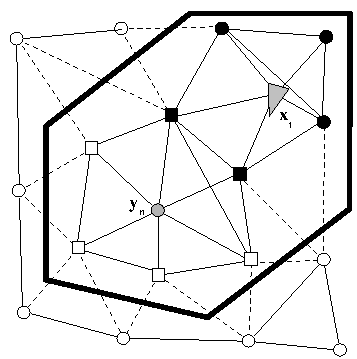
\includegraphics[]{figs/pb-markov-blanket}
  \caption[Visualização da rede formada entre o robô e os \textit{landmarks}]{Rede de conexões entre \textit{landmarks} e o robô. A maioria das \textit{landmarks} estão representadas por círculos, as \textit{landmarks} vizinhas da \textit{landmark} candidata a associação estão representadas por quadrados. As \textit{landmarks} ativas estão coloridas de preto, a \textit{landmark} candidata está colorida de cinza. O polígono de bordas grossas delimita o conjunto do Cobertor de Markov, $\bsubvec{m}{c_t}^+$. Neste caso há interseção entre o conjunto de \textit{landmarks} vizinhas e ativas. Retirado de \cite[p.~410]{thrun2005probabilistic}.}
  \label{fig:markov-blanket}
\end{figure}

Utilizando o resultado do condicionamento da distribuição gaussiana na forma de 
informação apresentado no Anexo \ref{annex:info-gaussian-conditioning} e já 
utilizado na esparsificação, calcula-se a matriz de covariância aproximada $\approxcov{\mathrm{m^j}}$ da seguinte forma:
\begin{equation}
  \approxcov{\mathrm{m^j}} = \proj{\mathrm{m^j}} \parentheses{\proj{\robotstate{t}, \mathrm{m^j}, \bsubvec{m}{c_t}^+}\, \infom{t} \,\projT{\robotstate{t}, \mathrm{m^j}, \bsubvec{m}{c_t}^+}}^{-1} \projT{\mathrm{m^j}}
\end{equation}

Entretanto, ao contrário do que é mostrado na Figura \ref{fig:markov-blanket}, 
pode ser que não exista interseção entre o conjunto de \textit{landmarks} 
vizinhas a candidata e o conjunto de \textit{landmarks} ativas $\bupvec{m}{+}$ 
dentro do Cobertor de Markov. Nesses casos, o cobertor deve ser aumentado de 
forma que englobe um ``caminho'' entre o robô e a \textit{landmark} candidata. 
Para isso, a matriz de informação pode ser interpretada como um grafo e inserir 
as \textit{landmarks} que integram o menor caminho entre o robô e a 
\textit{landmark} candidata.

\section{Estratégia para mitigar efeito de falsas detecções de \textit{landmarks}}
\label{sec:false-detection-handling-strategy}
Um problema comum que ocorre na prática em sistemas SLAM é a detecção 
errônea e/ou falsa de \textit{landmarks} gerando medidas erradas. Isso pode 
acontecer por erros no processamento dos dados do sensor, movimentos bruscos 
do robô, e em sistemas multiagentes um robô pode ser confundido com uma \textit{landmark} dependendo dos tipos de \textit{landmark} e do sensor utilizado. 
Esse último é particularmente comum no cenário desse trabalho, onde as \textit{landmarks} e os robôs possuem formato cilíndrico e o sensor do tipo LiDAR 
fornece apenas informação espacial, sem cores ou texturas.

Falsas detecções podem levar a falsas associações de novas medidas, 
acarretando em erro de localização e consequente divergência na 
observação de novas \textit{landmarks}. Para atenuar esse problema e 
diminuir as chances de uma falsa \textit{landmark} causar 
divergência dos filtros, é comum separar as \textit{landmarks} em uma lista provisória e numa lista permanente.

A lista de \textit{landmarks} permanentes é composta pelas 
\textit{landmarks} já consolidadas pelo filtro, e influenciam 
na estimação da pose do robô. Já as \textit{landmarks} 
provisórias são \textit{landmarks} ainda não consolidadas; as leituras 
associadas a elas são utilizadas apenas para melhorar a estimativa de 
suas posições e não influenciam na estimação da pose do robô.

Para construir essas listas \citeonline{saputra2019implementation} empregou 
o uso de um esquema de pontuação para as 
\textit{landmarks} observadas. Esse esquema possui duas operações: 
atualização e degradação. A operação de atualização consiste em 
aumentar um ponto a pontuação $\mathcal{Q}$ da \textit{landmark} sempre que ela 
é reobservada. Enquanto a degradação diminui dois pontos sempre que a 
\textit{landmark} não é reobservada.
\begin{equation}
  \lscore{t+1}{j} = \begin{cases}
    \bupvec{m}{j}\, \text{é reobservada} &\implies \lscore{t}{j} + 1 \,\, \text{(atualização)}\\
    \bupvec{m}{j}\, \text{não é reobservada} &\implies \lscore{t}{j} - 2 \,\, \text{(degradação)}\\
  \end{cases}
  \label{eq:landmark-quality}
\end{equation}
Toda \textit{landmark} começa na lista provisória e conforme sua 
pontuação $\mathcal{Q}$ evolui no tempo ela pode ser promovida para a 
lista de \textit{landmarks} permanentes, passando a ser utilizada na 
correção da pose do robô. Ou até mesmo removida no filtro caso deixe de 
ser observada sistematicamente. Uma \textit{landmark} se torna 
permanente quando sua pontuação chega a 10, e é excluída quando pontua 
cinco pontos negativamente:
\begin{equation}
  \begin{cases}
    \lscore{t}{j} \geq 10 & \text{Promoção}\\
    \lscore{t}{j} \leq -5 & \text{Remoção}\\
  \end{cases} 
\end{equation}

Com essa abordagem foi possível erradicar a incorporação de 
falsas \textit{landmarks} geradas tanto no cenário com um robô quanto 
no cenário com dois robôs. Além disso, como será visto na Seção \ref{sec:seif-map-exchange}, ao trocarem seus mapas os robôs enviam para o 
outro par apenas o vetor e matriz de informação correspondentes às 
\textit{landmarks} consolidadas pelo filtro (i.e. permanentes).

\section{Conclusão do capítulo}
Neste Capítulo foram exploradas as particularidades da estimação de 
estado de sistemas SLAM em relação à estimação de estado de sistemas 
convencionais. Enquanto um sistema SLAM possui vetor de estados com 
tamanho dinâmico, o tamanho do vetor de medidas é variante no tempo, uma porção do estado é variante no tempo (a pose do robô) enquanto a 
outra é invariante (posição das \textit{landmarks}), e a associação 
entre medidas e estados é desconhecida a \textit{priori}. Um sistema convencional possui número de medidas fixo e os componentes do estado têm mesmo 
tipo de variabilidade no tempo. 

Também foram mostradas as adaptações necessárias para utilizar o 
Filtro de Kalman Estendido na estimação de estado de sistemas SLAM, 
caracterizando a técnica EKF-SLAM. Além disso, foi apresentado a técnica 
SEIF-SLAM e como ela é baseada na formulação dual do EKF, e como 
ela utiliza o conceito de \textit{landmarks} ativas para manter a 
matriz de informação esparsa levando ao uso linear de memória e tempos 
de atualização e predição constantes. Mais adiante, na Seção \ref{sec:seif-map-exchange} também será mostrado como a troca de informações 
entre sistemas SEIF-SLAM é natural devido a utilização da parametrização 
canônica do filtro.

Além disso foi abordada a técnica de associação de dados 
\textit{Individual Compatibility Nearest Neighbor}, efetiva no ambiente deste trabalho. E por fim, foi tratado o problema prático da detecção 
de falsas \textit{landmarks} e como atenuá-lo.
